\documentclass{article}
\usepackage[utf8]{inputenc}
\usepackage[margin=1in]{geometry}
\usepackage{pdfpages}
\usepackage{hyperref}

\hypersetup{
	hidelinks,
	backref,
	pdftex,
	pdfauthor={Kevin Kässens and Enno Teßmer},
	pdftitle={Project Report: How does BERT answer questions?}
}

\title{Project Report: How does BERT answer questions?}
\author{Kevin Kässens, Enno Teßmer}
\date{Deep Learning 2021}

\begin{document}
	\maketitle
	\section{Introduction}
	In this report, we present the results we achieved while working on our Deep Learning project. For our self-written code and any other additional files, we created a GitHub repository that can be found at \url{https://github.com/UNF-B5S/dl-project}.\\
	
	The goal of our project was to study BERT and to understand how BERT manages to answer a given question. 
	
	\section{Reproduced}
	\subsection{Visualization}
	We reproduced the visualization results using the hidden\_state\_visualizer.py script from the explain-BERT-QA repository. We used the SQuAD and bAbI models from the VisBERT models and created the samples with the question, answer and context according to the examples in the paper.
	You can find samples from our results in the figures below. In the last figure of both examples, it is clearly visible that BERT was able to extract the correct answer to the question in both cases.
	
	To see the plot for each hidden layer of an example, check the subfolder corresponding to the example in ./badges/reproduced/visualization.
	
	\subsubsection{SQuAD example}
	
	\begin{tabular}{ l p{0.85\linewidth} }
		Question: & What is a common punishment in the UK and Ireland? \\
		Answer: & detention \\
		Context: & Currently detention is one of the most common punishments in schools in the United States, the UK, Ireland, Singapore and other countries. It requires the pupil to remain in school at a given time in the school day (such as lunch, recess or after school); or even to attend school on a non-school day, e.g. "Saturday detention" held at some schools. During detention, students normally have to sit in a classroom and do work, write lines or a punishment essay, or sit quietly. \\
	\end{tabular}
	
	\begin{center}
		\begin{tabular}{ c c }
			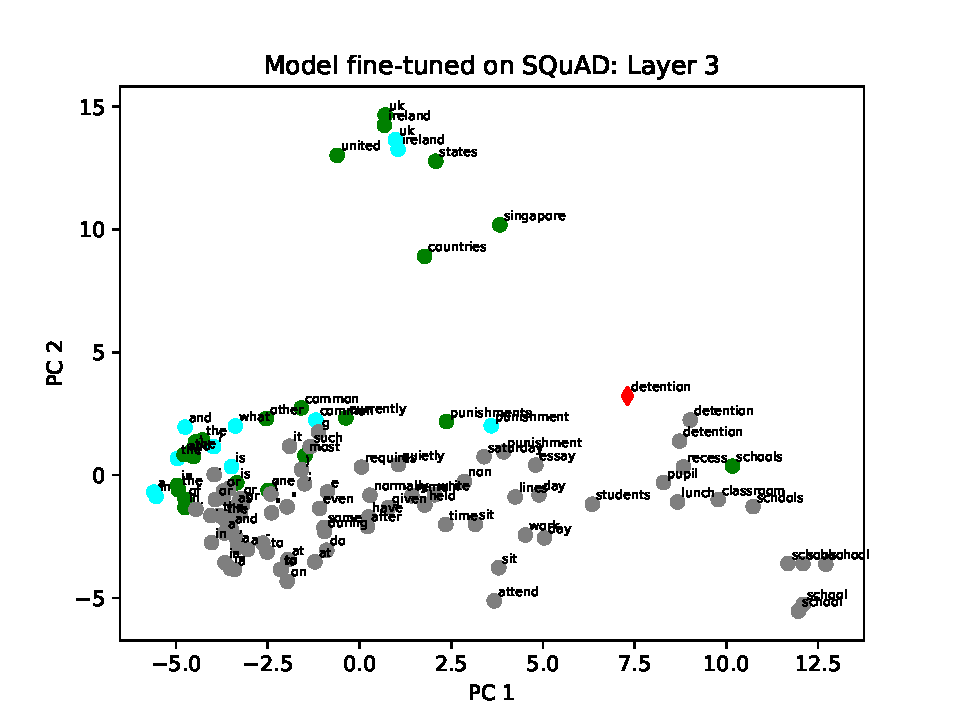
\includegraphics[scale=0.4]{../badges/reproduced/visualization/squad/model-fine-tuned-on-squad--layer-3.pdf} &
			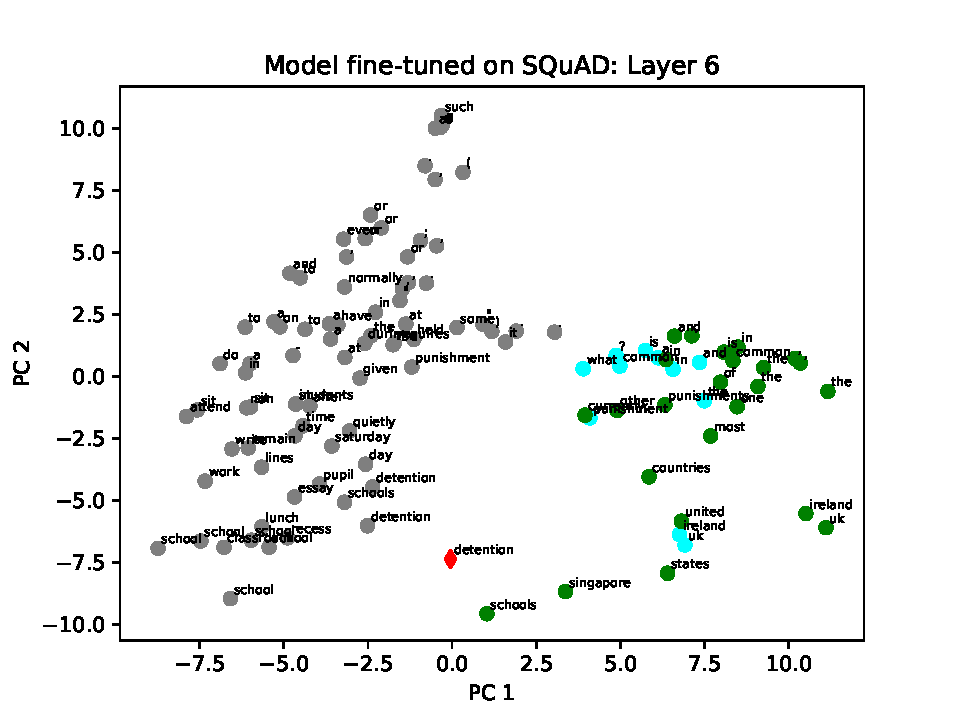
\includegraphics[scale=0.4]{../badges/reproduced/visualization/squad/model-fine-tuned-on-squad--layer-6.pdf}
		\end{tabular}
	\end{center}

	\begin{center}
		\begin{tabular}{ c c }
			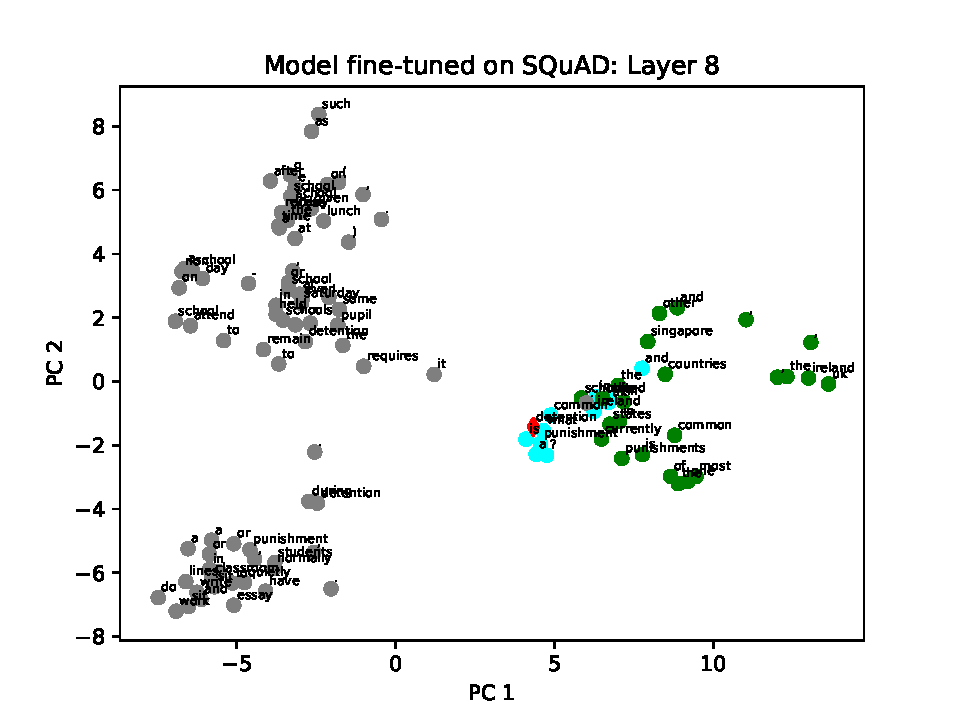
\includegraphics[scale=0.4]{../badges/reproduced/visualization/squad/model-fine-tuned-on-squad--layer-8.pdf} &
			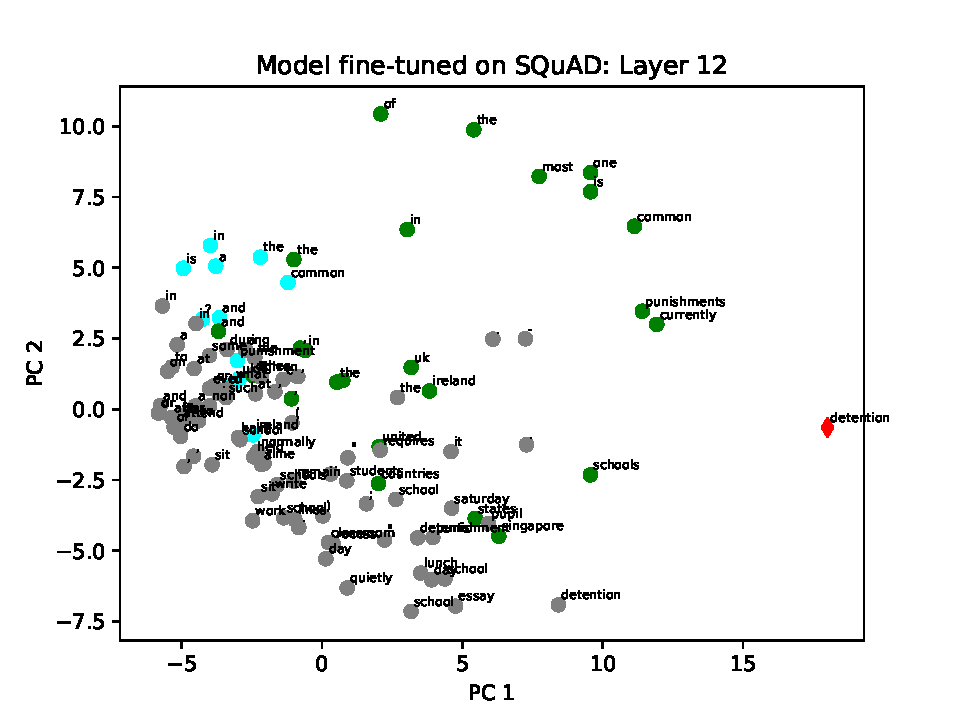
\includegraphics[scale=0.4]{../badges/reproduced/visualization/squad/model-fine-tuned-on-squad--layer-12.pdf}
		\end{tabular}
	\end{center}

	\subsubsection{bAbI example}

	\begin{tabular}{ l p{0.85\linewidth} }
		Question: & What is Emily afraid of? \\
		Answer: & cats \\
		Context: & Wolves are afraid of cats. 
		
		Sheep are afraid of wolves. 
		
		Mice are afraid of sheep. 
		
		Gertrude is a mouse. 
		
		Jessica is a mouse. 
		
		Emily is a wolf. 
		
		Cats are afraid of sheep. 
		
		Winona is a wolf. \\
	\end{tabular}
	
	\begin{center}
		\begin{tabular}{ c c }
			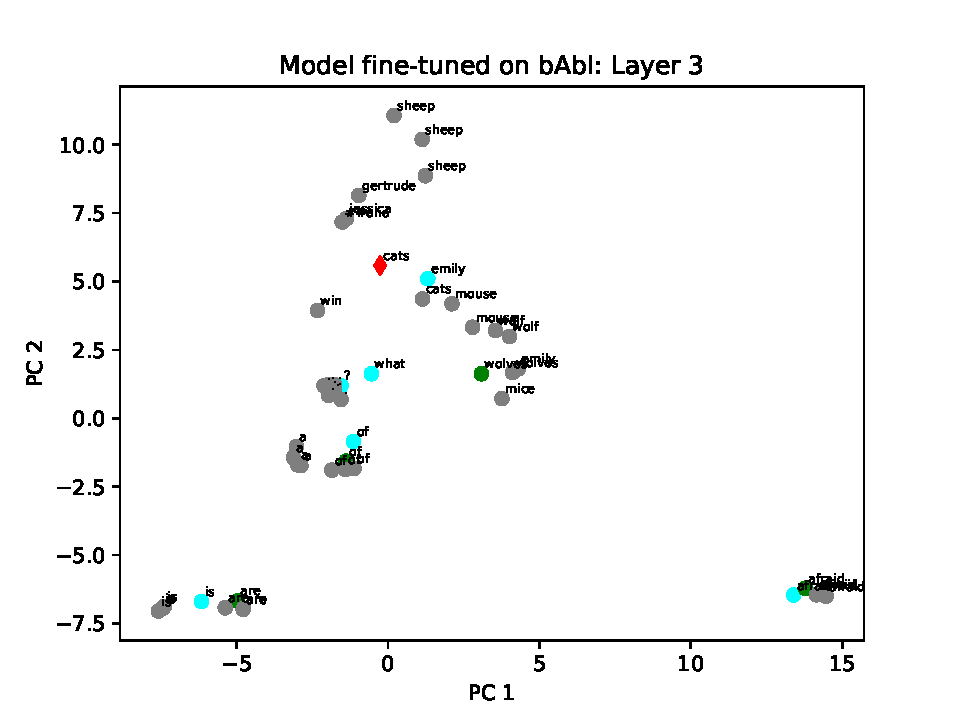
\includegraphics[scale=0.4]{../badges/reproduced/visualization/babi/model-fine-tuned-on-babi--layer-3.pdf} &
			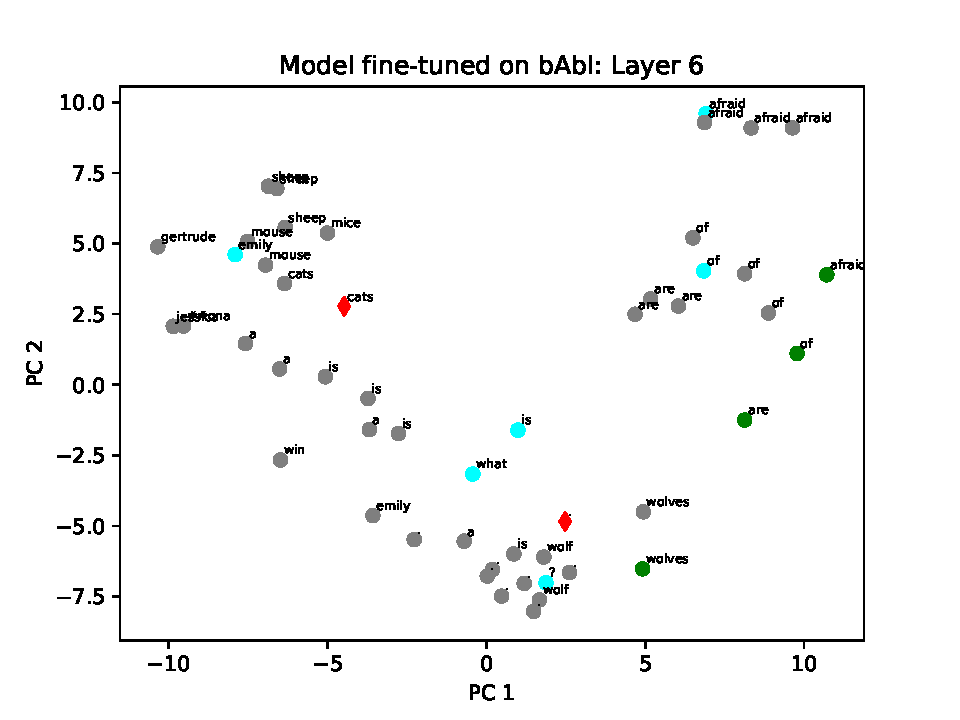
\includegraphics[scale=0.4]{../badges/reproduced/visualization/babi/model-fine-tuned-on-babi--layer-6.pdf} 
		\end{tabular}
	\end{center}

	\begin{center}
		\begin{tabular}{ c c }
			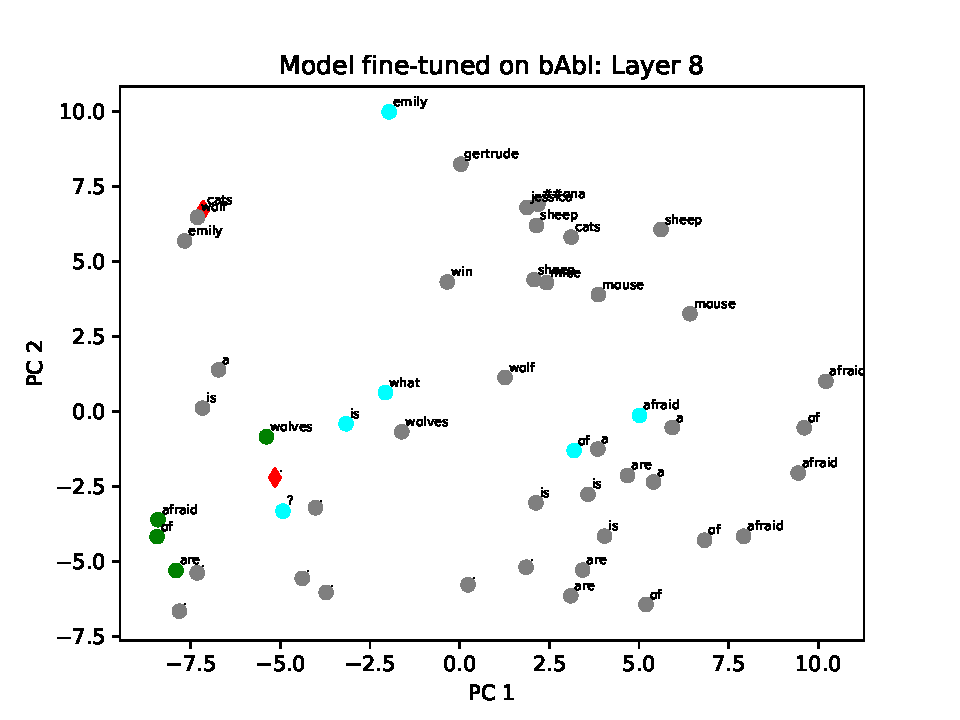
\includegraphics[scale=0.4]{../badges/reproduced/visualization/babi/model-fine-tuned-on-babi--layer-8.pdf} &
			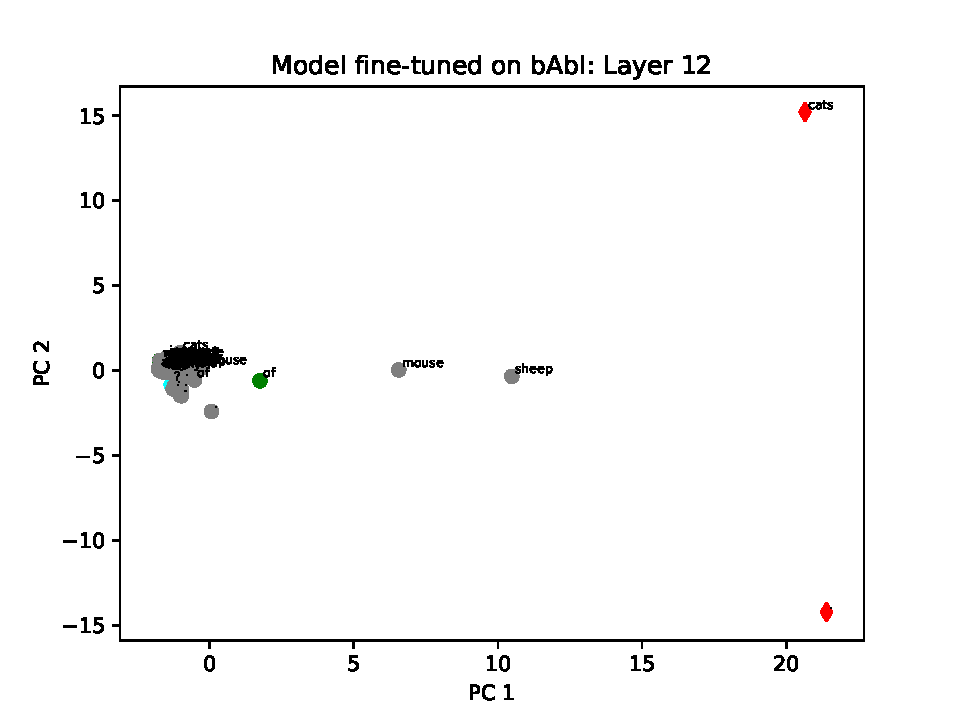
\includegraphics[scale=0.4]{../badges/reproduced/visualization/babi/model-fine-tuned-on-babi--layer-12.pdf}
		\end{tabular}
	\end{center}

	\subsection{Probing}
	Despite our best efforts, we were not able to get the Jiant Probing Suite set up and running and therefore could not reproduce the probing results from the paper. \\
	
	We initially tried to set up Jiant on Windows 10, but had no success. We received various errors we eventually were not able to resolve. Therefore, we instead tried using a virtual machine running Linux (Ubuntu). Although we did have more success on Linux than on Windows and managed to progress further in the installation and setup progress, we were still not able to get Jiant fully set up. Eventually we again received an error we were not able to resolve and hence could not progress any further. 
	
	Details about the error we received when we tried to run any of the experiments from the paper can be found below:\\
	
	We registered a new task in the edge\_probing.py file and set all paths correctly. We added the task we registered as the target task in the config file and set the input module to "bert-base-uncased". But when we ran the main.py script with this config file, we received the error "input length exceeds position embedding capacity, reduce max\_seq\_len" on the "Evaluating model on tasks" step. 
	
	The value used for max\_seq\_len in the bert\_edgeprobe.conf is 512. We tried reducing the value in the config file to different values, as well as using the value from the defaults.conf file, but none of these changes solved the problem.\\
	
	We discovered that this exact problem was discussed in multiple entries under the Issues tab on the jiant-v1-legacy GitHub repository. Sadly, none of these discussions offered an explanation or a solution to our problem. The majority of these discussions were automatically closed for the reason that the old version of Jiant will no longer be supported.
	
	With the documentation of the Jiant Probing Suite being rather sparsely, we were not able to find a solution to our problem or make any other progress on our own.\\
	
	We tried using the new version of the Jiant Probing Suite as well. But we had no luck with this version either.\\
	
	After over 40 hours of unsuccessfully trying to set-up Jiant, we decided it would be more promising for us to work on other badges instead.
	
	\section{Replicated}
	\subsection{Visualization}
	You can find our script that creates the visualizations for the hidden layers in the folder ./badges/replicated/visualization.\\
	
	The main script is visualization.py. The other script, visualization\_classes.py only holds the class definitions for the main script.
	
	To run our script, call the visualization.py. It accepts the following command line arguments:
	
	\begin{itemize}
		\item -sample: Path to the sample file
		\item -model: Path to the model file
		\item -type: Type of the model (optional, default: bert-base-uncased)
		\item -title: Title of the experiment (optional)
		\item -format: File format for the output (png,pdf,svg,jpg) (optional, default: png)
		\item --no-legend: If set, no legend will be added to the plots
	\end{itemize}

	The results will be saved to a subfolder of ./outputs, named like the experiment's title (set with -title`option). If the title of the experiment is not set, the current date and time will be used instead.\\

	
	You can find an example output from our script below. This is the plot our script generates for the squad sample from the paper. To see the plots for the other layers, as well as the results for the bAbI example, check the folder ./badges/replicated/visualization/output.
	
	\begin{center}
		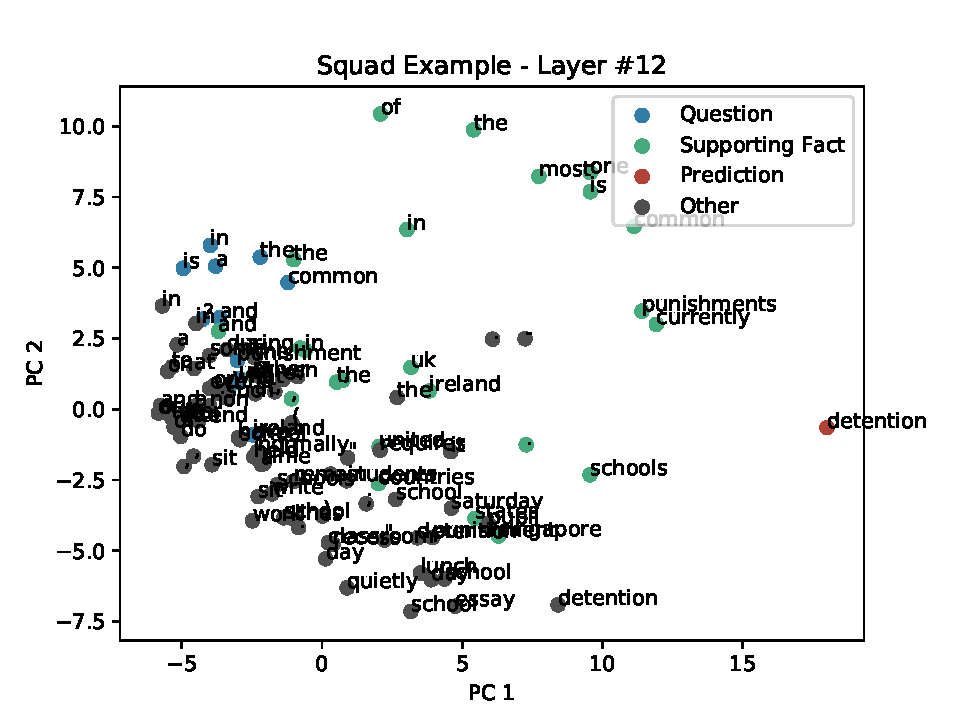
\includegraphics[scale=0.6]{../badges/replicated/visualization/output/squad-example/layer-12.pdf}
	\end{center}
	
	\section{New Code Variant}
	While experimenting with the visualization script from the explain-BERT-QA we discovered that it does not work well when the sample's context is longer than BERT's maximum length.\\
	
	Although the script implements a sliding window approach to handle such inputs, it always processes the first window that it generates.
	
	The reason for that is in the data\_utils.py script. In the function “convert\_qa\_example\_to\_features“ starting at line 226, the windows are generated. After that a for-loop is used to iterate through all windows (line 239). But at the end of this loop, a return statement always terminates the loop (line 359). There are no continue statements prior to the return statement in the loop either, so the loop always terminates after the first iteration by returning the first window.
	
	If the answer is not within this window, the script prints that the given example is impossible and creates useless visualizations.\\
	
	Therefore, we modified the code in a way, that the script returns useable results, even when the answer is not in the first window.
	
	To achieve that, all windows will be processed and given to BERT. Eventually, only the window where BERT’s prediction has the highest probability will be visualized. 
	
	You can find our modified code in ./badges/new-code-variant/visualization. All places where we modified or added some code are marked with a comment starting with "\# ADDED", as well as a short explanation of what we did.\\
	
	To reproduce this experiment, we created an additional sample, "sample\_squad\_long.json". You can find it in the folder ./badges/new-code-variant/visualization. This sample contains an excerpt from the Wikipedia article about Gottfried Wilhelm Leibniz at the beginning of the context, so no information that is relevant for the question "What is a common punishment in the UK and Ireland?".
	
	While the original script, given this sample, does not create useful results, our modified script is able to give the correct answer ("detention") to the question.
	
	
\end{document}
